\section{Full Experiments on Dense Potentials}
\label{app:potentials}

The main text treats the dense progress \emph{potential} as the reachability-gated half of the process signal (\S\ref{sec:potentials}). This appendix gives the full experiments. The picture is consistent with the variance account: where a potential's intermediate values are \emph{reachable} it supplies gradient the outcome lacks and accelerates training, and where they are unreachable it is exactly vacuous. Converting the extra gradient into a stable success gain requires a bounded optimizer---an aggressive update rule can destabilize the densely shaped policy, an optimization caveat we return to in \S\ref{app:fragility}. Unless noted, we train Qwen3~\citep{qwen3} with our own GRPO, place any dense credit on the responsible tokens with a separate per-channel normalizer, and count efficiency in \emph{episodes generated} so that resampling costs are visible.

\subsection{Reachability is measurable before training, and it gates the benefit}
\label{app:reachability}

The condition the variance account makes operative is reachability: a potential $\Phi$ helps only where the policy realizes differing intermediate values across a group, i.e.\ $\operatorname{Var}_G(\Phi)>0$. This can be checked \emph{before} spending training compute, from a handful of base-policy rollouts.

On SWE-bench software repair~\citep{swebench} the natural potential is the fraction of hidden \texttt{FAIL\_TO\_PASS} tests an episode makes pass. Two facts make it vacuous (Figure~\ref{fig:reachability}). Structurally the finer potential barely exists: two-thirds of instances have a single failing test, so $\Phi$ collapses to the binary outcome, and only a third admit any partial progress. Empirically even that third is unreachable: across $156$ rollouts of a $30$B policy \emph{every} episode scores $\Phi=0$, so $\operatorname{Var}_G(\Phi)$ is identically zero and a $\Phi$-based reward centers out to no gradient. The cause is not gameability but unreachability---there is no realized intermediate state for any reward to act on.

Mapping the same no-training proxy $\operatorname{Var}_G(\Phi)$ across model capability ($0.6$--$4$B) and outcome sparsity (Figure~\ref{fig:phase}a) reproduces the structure the account predicts: it rises with capability and peaks in the sparse-but-reachable corner. The measured dense-reward benefit tracks it (Figure~\ref{fig:phase}b): $\approx\!0$ where $\operatorname{Var}_G(\Phi)\!\approx\!0$ (the SWE null; the too-weak small models) and large where it is high (the $4$B reachable chain, dense $0.34$ vs.\ outcome $0.01$; real theorem proving, below). Benefit appears only past a reachability threshold. We could not fill the map's interior with controlled \emph{training} points---small-scale synthetic training is too learning-rate-sensitive, most cells degenerating to zero for both arms---so the benefit axis rests on the real-domain anchors plus one clean controlled point.

\begin{figure}[tbp]
\centering
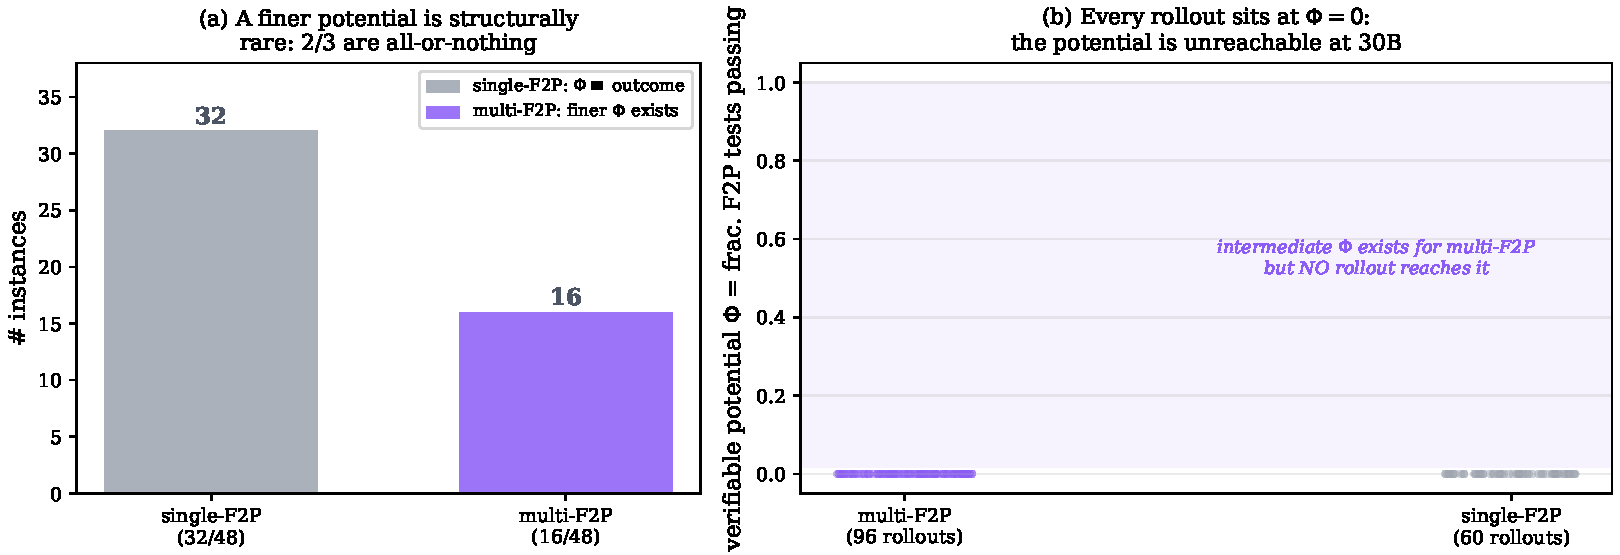
\includegraphics[width=\textwidth]{figures/fig_ec_reachability.pdf}
\caption{\textbf{In software repair the finer potential is structurally rare and empirically unreachable.} \emph{(a)} Of $48$ single-file-fix SWE-bench instances, two-thirds have a single failing test, so the test-fraction potential equals the binary outcome; only one-third admit a finer $\Phi$. \emph{(b)} For those, a $30$B policy's rollouts never realize it: all $156$ rollouts score $\Phi=0$. The band of intermediate values exists but is empty---zero within-group variance, hence zero gradient.}
\label{fig:reachability}
\end{figure}

\begin{figure}[tbp]
\centering
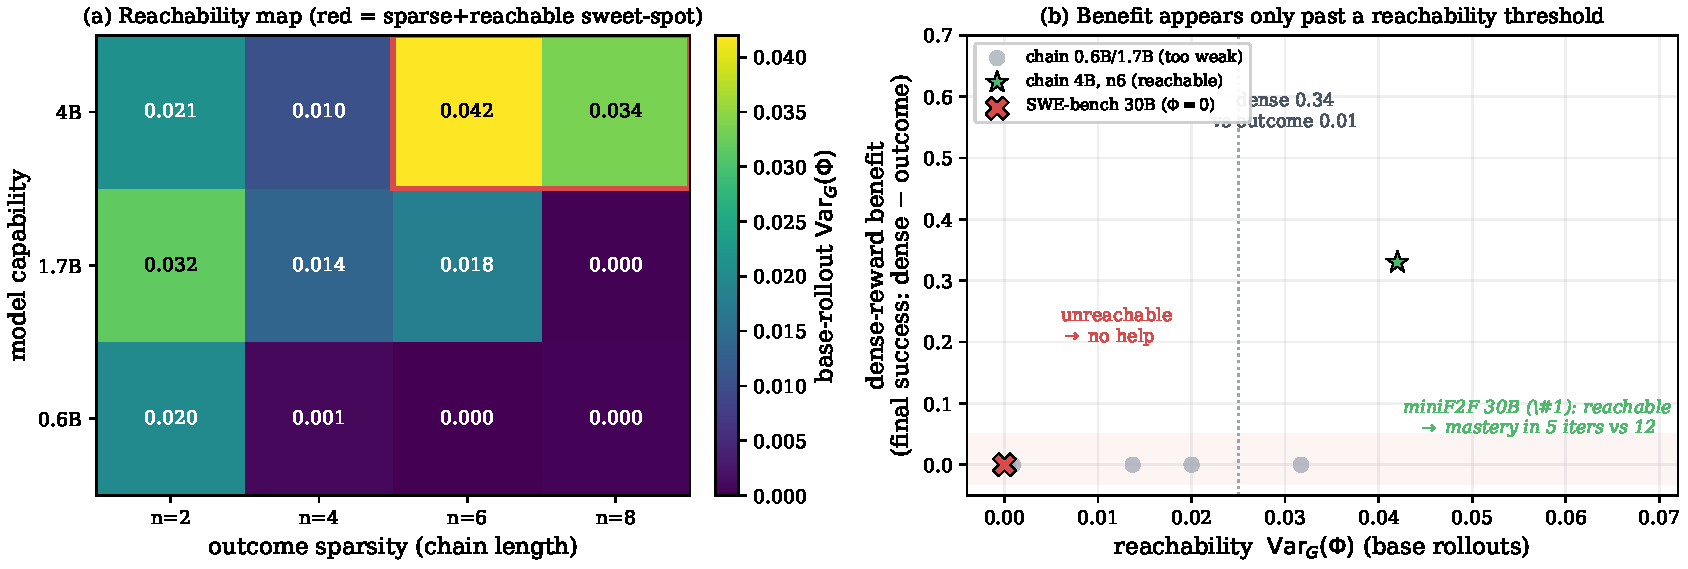
\includegraphics[width=\textwidth]{figures/fig_phase_diagram.pdf}
\caption{\textbf{Reachability, measured cheaply, gates the dense-reward benefit.} \emph{(a)} $\operatorname{Var}_G(\Phi)$ on base-policy rollouts (no training) over model capability $\times$ outcome sparsity: it rises with capability and peaks in the sparse-but-reachable corner. \emph{(b)} The benefit of a dense reward (final-success gap, dense $-$ outcome) against that same probe: zero where $\operatorname{Var}_G(\Phi)\!\approx\!0$ and large where it is high. Benefit appears only past a reachability threshold.}
\label{fig:phase}
\end{figure}

\subsection{Where the potential is reachable, it removes dead updates and accelerates}
\label{app:efficiency}

When the potential's intermediate values are reachable and point the same way as success, a dense signal is genuinely useful. We instantiate it on a family of \emph{$N$-stage chained} file-operations tasks (tools \texttt{list\_dir}, \texttt{read\_file}, \texttt{write\_file}, \texttt{delete}, \texttt{run\_tests}, \texttt{submit}); success requires all $N$ stages, so $N$ tunes base difficulty ($N{=}4$ sits near $8\%$ base success). The dense signal is a verifiable progress potential carried on a token-attached channel (a penalty when a call violates a rule---overwrite a file never read, submit an untested change---and a credit when a call discharges a pending obligation).

\paragraph{Dead updates.} We count the fraction of iterations whose update is \emph{dead}: an all-fail group with no reward spread (Figure~\ref{fig:paired}). Outcome-only GRPO is dead on $65\%$ of iterations. DAPO~\citep{dapo}, built to dodge all-fail groups by resampling, reaches $54\%$ but pays a $5.6\times$ generation tax. The aligned potential cuts dead updates to $8\%$ at no extra sampling, by producing gradient from the very failures the outcome reduces to zero. The cure is the credit scheme, not the budget---and it is contingent on reachability: on the silent-precondition gate (\S\ref{app:ceiling}), where the pivotal action is never sampled, every reward-only method is dead almost always (outcome and DAPO $100\%$, the potential $76\%$), because a discharge can fire only on behavior the policy attempts.

\paragraph{Speed.} On held-out success against episodes generated (Figures~\ref{fig:efficiency},~\ref{fig:seeds}) outcome-only crawls, spending its budget on dead updates, then converges only at the end; the aligned potential rises immediately from the early all-fail groups. Reimplemented dense baselines (GiGPO-style step advantages~\citep{gigpo}, StepTool-style per-call rewards~\citep{steptool}) also outpace outcome-only---any \emph{admissible} dense signal helps. The gain also holds on real theorems (miniF2F~\citep{minif2f}) at 4B and 30B, but only in the multi-seed form quantified in \S\ref{app:fragility}: a single-run pilot of ours showed a dramatic $2.4\times$ speed-up that \emph{flipped sign} when the identical configuration was re-run (rollout sampling is unseeded in the serving engine, and MoE training at this scale is bimodal), so we report only the five-seed matrix (Figure~\ref{fig:recipescale}, Table~\ref{tab:p0}): a $\sim$1.6$\times$ speed-up to mastery under a matched optimizer, consistent on every seed, plus the reliability advantage. Both arms saturate---the claim is speed and reliability, not final success.

\begin{figure}[tbp]
\centering
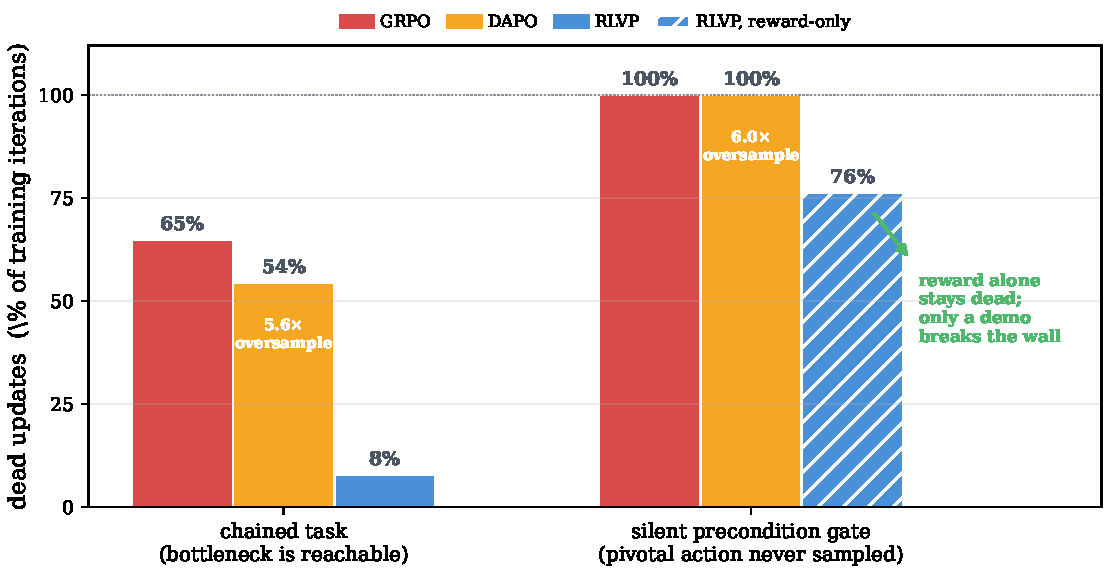
\includegraphics[width=0.84\textwidth]{figures/fig_paired_dead.pdf}
\caption{\textbf{Dead updates across two regimes.} Fraction of iterations with an all-fail, zero-spread group (Qwen3-4B, 3-seed mean). \emph{Chained task} (bottleneck reachable): outcome-only $65\%$, DAPO $54\%$ at a $5.6\times$ generation tax, the aligned potential $8\%$. \emph{Silent precondition gate} (\S\ref{app:ceiling}, pivotal action never sampled): outcome and DAPO dead on \emph{every} iteration, the reward-only potential $76\%$; only a demonstration seed breaks the wall. The cure is a \emph{reachable, admissible} signal, not density.}
\label{fig:paired}
\end{figure}

\begin{figure}[tbp]
\centering
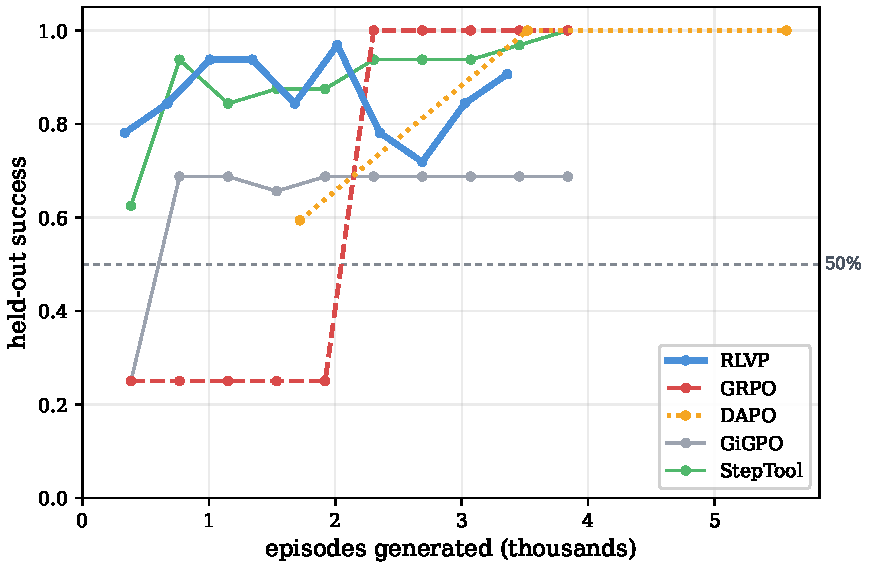
\includegraphics[width=0.9\textwidth]{figures/fig_efficiency.pdf}
\caption{\textbf{Sample efficiency on the calibrated hard task ($N{=}4$).} Held-out success vs.\ episodes generated. Outcome-only sits near base rate for most of training; the aligned potential climbs immediately from the all-fail groups; dense baselines also outpace outcome-only. The $x$-axis counts episodes \emph{generated}, including DAPO's resampling.}
\label{fig:efficiency}
\end{figure}

\begin{figure}[tbp]
\centering
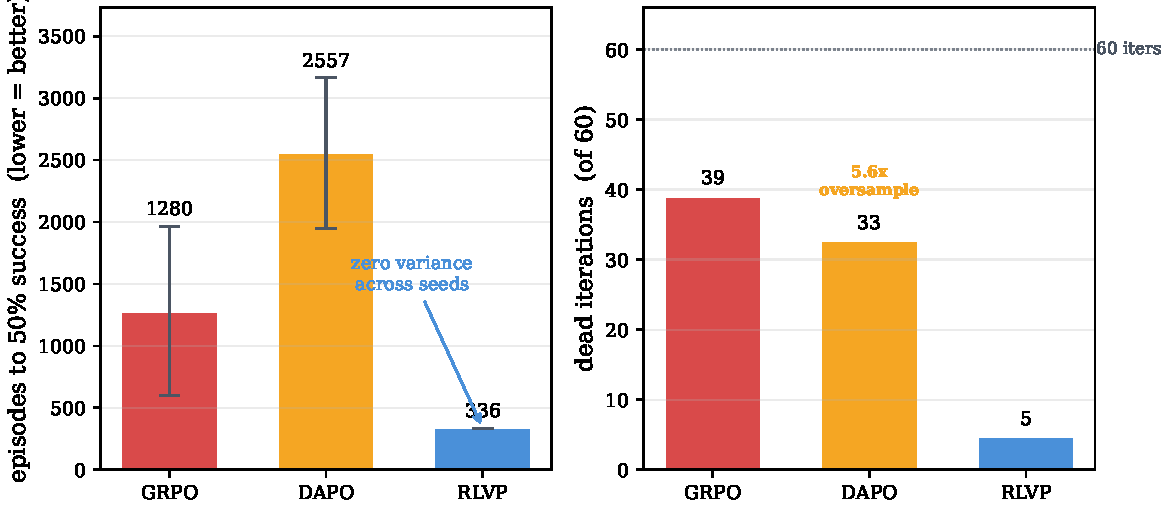
\includegraphics[width=\textwidth]{figures/fig_seeds.pdf}
\caption{\textbf{Efficiency over three seeds.} \emph{Left:} episodes to the success threshold (lower better)---the potential is several times faster than GRPO and DAPO. \emph{Right:} the mechanism---GRPO and DAPO burn most iterations on dead or stalled updates, and DAPO generates $5.6\times$ the episodes it uses. Note the large GRPO error bar: the all-fail lottery on the outcome side, which the dense potential's reachable within-group variance avoids.}
\label{fig:seeds}
\end{figure}

\subsection{Converting the gradient to success: protocol, and the matched matrix}
\label{app:fragility}

The extra gradient a reachable potential supplies must still be turned into task success, and here the decisive factor is the optimizer, not the potential. Early runs read this as ``fragility,'' but the cause was two experimental artifacts. First, an aggressive, unbounded update rule can destabilize a densely shaped policy: at one fixed learning rate, a theorem-proving run anneals cleanly to full success (gradient norm $<1.5$, entropy decaying to zero) while an otherwise-identical sibling suffers a gradient blow-up (norm $>10^{9}$), its entropy explodes, and success collapses to zero and never recovers---the same signal, the same rate, decided by optimization stability. On the chained task the opposite failure appears: the policy collapses to a zero-entropy degenerate output, so every rollout is identical, the within-group variance is zero, and the update dies. A \emph{bounded} optimizer (we use Muon, with a divergence guard that aborts on entropy collapse or gradient spikes) removes both failure modes. Second, per-iteration training success measured on a handful of freshly sampled tasks is too noisy to read a speed-up from---it swings between extremes iteration to iteration---so we evaluate on a fixed held-out task set. The result robust to all of this---the mechanism the paper relies on---is dead-update elimination: zero dead iterations against $\sim$16 of 40 for outcome-only, on \emph{every} seed.

\paragraph{The matched matrix: five seeds, two scales.} With the bounded-optimizer protocol fixed (aligned goal-progress potential as a token-attached discharge, Muon, a divergence guard, $30$ iterations on miniF2F algebra), we ran the full matrix---aligned potential versus outcome-only, five seeds per arm, at 4B and 30B, plus a three-seed anneal ablation and a 30B AdamW outcome baseline; all magnitudes are in Table~\ref{tab:p0}. Because rollout sampling in the serving engine is unseeded, ``seeds'' are i.i.d.\ draws of the whole run, so per-arm consistency is the meaningful statistic. Three facts are seed-robust. \textbf{(1)~A modest, consistent speed-up} under a matched optimizer: the aligned potential reaches the threshold sooner and has higher area-under-curve on every seed-matched pair at 4B. \textbf{(2)~Reliability:} it completes every run across both scales without a divergence abort, while outcome-only loses seeds to entropy collapse (4B) and gradient explosion (30B)---the dense, always-relevant gradient appears to \emph{regularize} where the bursty sparse signal blows up under the same rate. \textbf{(3)~The outcome arm's dilemma at 30B:} outcome-only is competitive under the fast optimizer only when it survives (it diverges on most seeds), and stable under its safe optimizer only at several times the potential's time-to-mastery. The aligned potential requires no such choice.

\paragraph{Anatomy of the gain.} When the potential does win, ablating on $N{=}4$ (Figure~\ref{fig:ablationpot}) attributes the speed to the token-attached channel: folding the same rule rewards into the scalar return doubles the episodes to threshold. Annealing the shaping off after saturation protects the final ceiling (unrelaxed pressure drifts the policy toward over-compliant, bloated episodes---a mild inaction-trap tendency). The discharge credit is the positive signal that escapes all-fail groups; removing it leaves more dead iterations and a lower ceiling. Finally, replacing every hand-written rule with three universal meta-rules derived only from per-tool category tags (observe/mutate/verify/terminal) and the environment's error codes recovers the hand-engineered efficiency almost exactly: in well-structured environments the specification cost can be paid by metadata the tool schemas already expose.

\begin{figure}[tbp]
\centering
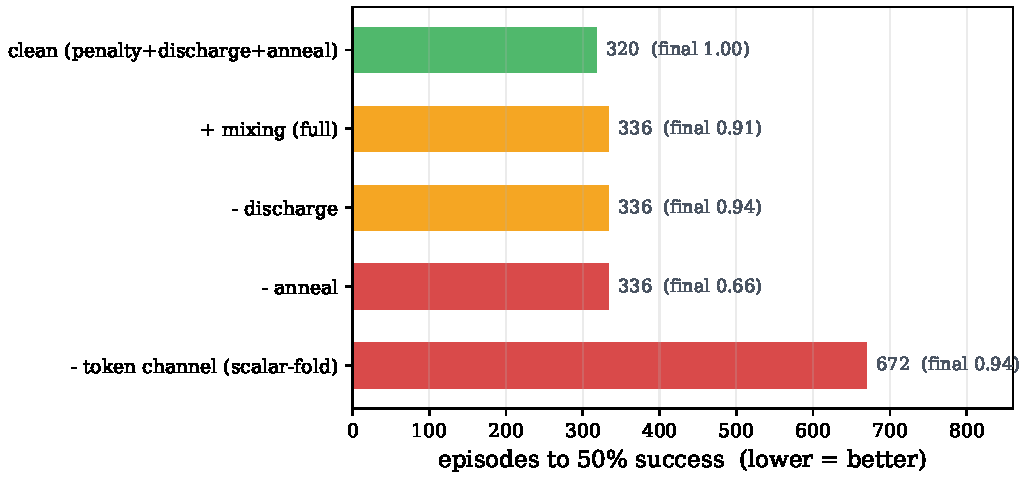
\includegraphics[width=0.92\textwidth]{figures/fig_ablation.pdf}
\caption{\textbf{Component attribution for the potential on $N{=}4$} (episodes to threshold, converged success annotated). The token-attached credit channel is the efficiency lever (folding into a scalar return doubles the cost); annealing protects the ceiling; the clean recipe is best. A per-step length cost, useful only on very long horizons, hurts here.}
\label{fig:ablationpot}
\end{figure}

\subsection{Reachability governs the ceiling, not just the speed}
\label{app:ceiling}

Sample efficiency is speed to a ceiling the chained tasks eventually reach. To ask whether a process reward can raise the \emph{ceiling}, we build a task that is hard to \emph{discover} rather than hard to compute: a \emph{silent precondition gate}, where to write a protected file the agent must first read an access-control file and request access; skip either and the write silently no-ops (reports success, does nothing). This is the bank-authentication problem of the introduction in controlled form---a required precondition an agent cannot stumble onto by trial and error and must be told---and it is where a purely reward-driven online learner would stall indefinitely. Calibration confirms the trap is total---the base model never reads the access file even when the rule is in its prompt. Then (Figure~\ref{fig:gated}) \emph{every} reward-only method (outcome, DAPO, the clean potential) fails to zero, because the discharge for reading the access file can only reward that behavior if the policy samples it, and it never does. A single rule-synthesized demonstration injected through the process channel breaks the wall to perfect, generalizing success. When the required behavior is never sampled, no on-policy reward can induce it; imitation must seed what reward then grows---the same reachability wall the SWE probe hit from the other side, and the R1-Zero (discoverable) versus R1 (demonstration cold-start) distinction in miniature.

\begin{figure}[tbp]
\centering
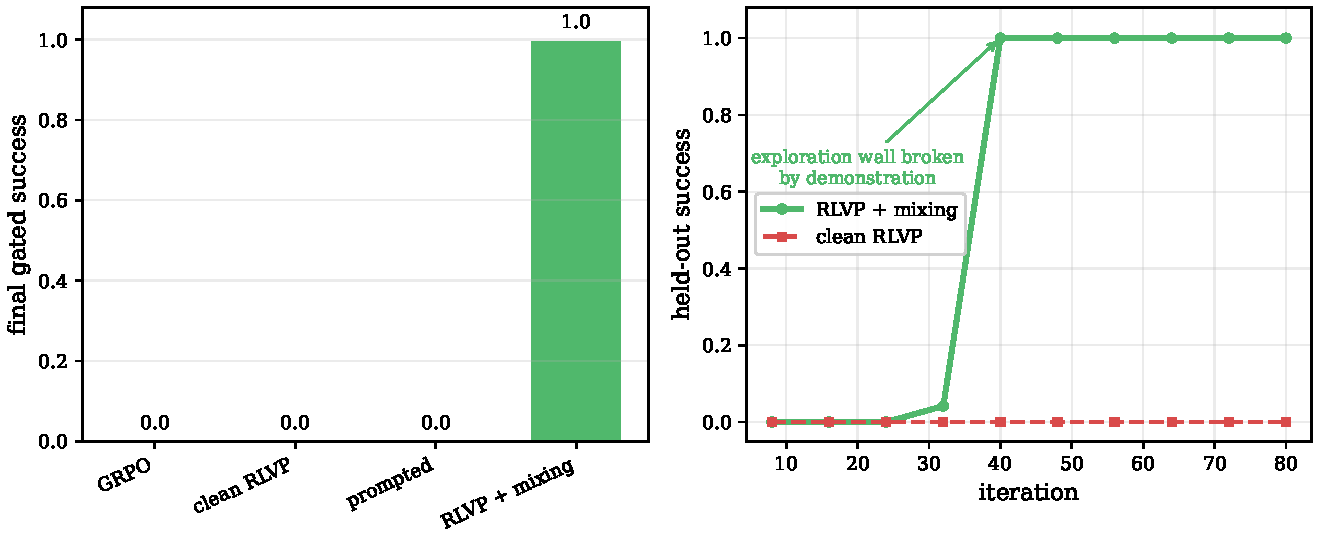
\includegraphics[width=0.96\textwidth]{figures/fig_gated_ceiling.pdf}
\caption{\textbf{A non-saturating ceiling test, and the discovery wall.} \emph{Left:} on the silent-gate task every reward-only method (outcome, DAPO, clean potential, even rules-in-prompt) converges to zero---the precondition is never sampled, so the discharge never fires. \emph{Right:} a single synthesized demonstration through the process channel breaks the wall to perfect held-out success, a sharp phase transition.}
\label{fig:gated}
\end{figure}

\subsection{Learning where the outcome is dead: real bug-fixing at zero success}
\label{app:deadcoding}

The variance account predicts that when a group is all-failing---outcome variance zero, outcome gradient dead---a process signal is the \emph{only} thing that can move the policy. We check this directly on real software repair, where an 8B agent is far below the task's reach. We train on SWE-smith~\citep{swesmith} instances (a repo container, a hidden \texttt{FAIL\_TO\_PASS} test as the oracle), with the agent issuing bash commands to find and fix the bug; the process channel is the coding-discipline signal of \S\ref{sec:path} (a discharge for running tests and making a verifiable edit, a penalty for re-running a failed command or editing without testing). At this scale the agent solves essentially \emph{zero} instances under either signal, so outcome-only RL trains on an all-fail distribution throughout---the cleanest possible test of the dead-gradient regime. This is a \emph{different} signal than the progress \emph{potential} of \S\ref{sec:potentials}: on this same software-repair domain the test-fraction potential is vacuous (Figure~\ref{fig:potentials}, left), because zero tests ever pass and so no intermediate value is reached. The penalized and discharged behaviors here---running a test, editing a file, re-running a failed command---are always reachable, so the penalty channel carries within-group variance exactly where the potential cannot. The two software-repair results are consistent: the reachability gate closes on the potential and stays open on the penalty.

The result is a sharp dissociation (Figure~\ref{fig:swetraj}, two seeds). Outcome-only leaves the trajectory \emph{flat}: productive actions per episode sit at $\approx\!1.5$ from the first iteration to the last, essentially identical across seeds ($1.5$ and $1.5$)---the dead gradient changes nothing. The process reward instead drives a steadily \emph{rising} trajectory: productive actions climb over training to $6.5$ and $11.4$ (final-3, the two seeds) and test-runs to $7.6$ and $12.9$, a four-to-tenfold increase, while the penalized behaviors fall (repeat-errors and untested edits toward zero). The agent learns to investigate, test, and edit like a disciplined engineer---from a signal available on every failed episode---exactly where the outcome reward is inert.

Two honest caveats scope the claim. First, the discharge \emph{rewards} test-running and productive edits, so part of their rise is by construction; the non-circular evidence is that the \emph{penalized} behaviors (which the discharge does not touch) also fall, and that the outcome baseline is perfectly flat---the effect is the process gradient, not the task. Second, this improved discipline did \emph{not} convert to task success in our budget (both arms remain at zero): 8B is simply too weak to close these bugs. The claim is therefore mechanistic and behavioral---the process channel produces learning, and better verifiable engineering discipline, precisely in the all-fail regime where outcome-only RL has no gradient at all---and a plausible precursor to success at capability, not a demonstration of success itself.

\begin{figure}[tbp]
\centering
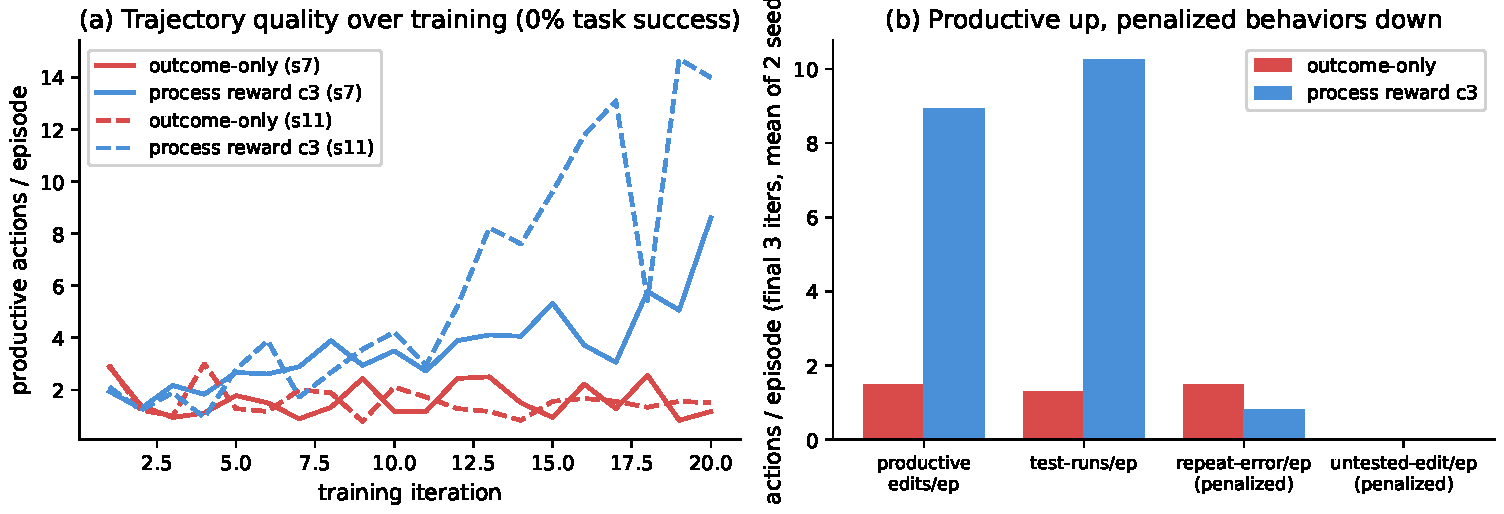
\includegraphics[width=\textwidth]{figures/fig_swesmith_traj.pdf}
\caption{\textbf{The process reward learns where the outcome is dead (SWE-smith, 8B, $\approx$0\% solve).} \emph{(a)} Productive actions per episode over training, two seeds: outcome-only is flat (the all-fail gradient is dead), while the process reward rises steadily. \emph{(b)} Final-3 trajectory quality (mean of two seeds): productive edits and test-runs increase several-fold under the process reward, while penalized behaviors (repeat-errors, untested edits) fall. Task success is zero for both arms throughout---this is a behavioral/mechanistic result, not a success result.}
\label{fig:swetraj}
\end{figure}


\section{Boundaries: When the Penalized Target Is Not Verifiable}
\label{app:boundaries}

Design rule~4 (\S\ref{sec:design}) requires the penalized (and discharged) target to be reachable and \emph{un-gameable}. This appendix gives the experiments behind that rule: what happens when a penalty's target is misaligned with the outcome, and when it is a \emph{learned} proxy rather than a verifiable predicate.

\subsection{An un-gameability sweep: which signals survive}
\label{app:sweep}

We construct five process signals for Lean theorem proving on miniF2F~\citep{minif2f}, spanning aligned to misaligned, pre-register each one's cheapest gaming policy, and train Qwen3-30B-A3B~\citep{qwen3} with each (three seeds, everything else fixed; Figure~\ref{fig:sweep}). Survival tracks admissibility. The \emph{penalty-free} signals reliably survive on every seed: a gameable ``any-valid-tactic'' credit, an aligned goal-progress discharge, and that credit \emph{gated on the eventual outcome} (un-gameable by construction, the most consistent survivor). The \emph{pure penalty}---an errored-tactic penalty with no discharge and no outcome reward---reliably \textbf{collapses to essentially zero on every seed}: its cheapest maximizer, avoid errors by not attempting, is precisely the \emph{inaction trap} of design rule~2, and with no positive signal to escape it the policy dies every time. This is the paper's cleanest evidence that a lone penalty cannot drive learning. The revealing case is \emph{penalty-plus-discharge}: across three seeds it is bimodal (collapses on two, rescued to perfect on the third), the largest variance of any arm---adding a discharge to a misaligned penalty makes survival \emph{possible} but not reliable. The robust reading: penalty-free progress signals survive, a pure penalty reliably collapses, and outcome-gating is the most consistent survivor. Precise magnitudes remain noisy at 30B; we report the survival pattern.

\begin{figure}[tbp]
\centering
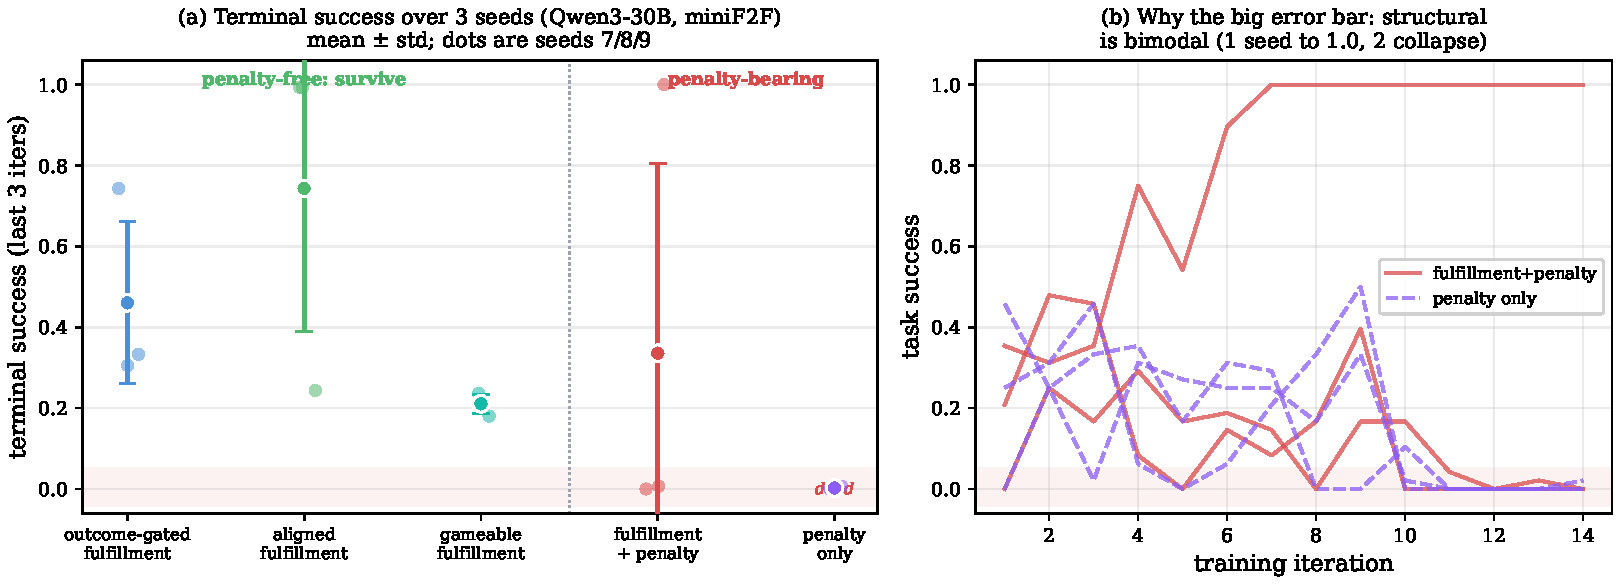
\includegraphics[width=\textwidth]{figures/fig_ungameability_sweep.pdf}
\caption{\textbf{Which signals survive (Qwen3-30B, miniF2F, 3 seeds).} \emph{(a)} Terminal success (last-3-iteration mean) for five signals, mean\,$\pm$\,std with seed dots. The three penalty-free signals sit well above the dead zone on every seed; the pure penalty is reliably dead; the discharge$+$penalty arm has by far the largest error bar. \emph{(b)} That arm is \emph{bimodal}---collapsing on two seeds, rescued to $1.0$ on one---whereas the pure penalty collapses on all three.}
\label{fig:sweep}
\end{figure}

\subsection{Task intent is not a verifiable rule}
\label{app:intent}

The hardest case for a penalty is a task whose difficulty is not procedural. On $\tau$-bench-style airline customer service~\citep{taubench} the reward turns on \emph{semantic} policy adherence (authorization, refund eligibility, confirmation) rather than structural ordering, so no verifiable rule is finer than the outcome: what is missing is intent, which is the reward itself. Three tiers make this concrete (Figure~\ref{fig:tau2}). \emph{Generic} structural rules---the read-before-write hygiene that works on chained tasks---are now orthogonal to the reward and actively \emph{harm}: the cheapest way never to violate ``confirm before calling'' is to not place the risky calls at all, and the policy collapses into the inaction trap within a handful of iterations. \emph{Policy-derived procedural} rules (fetch the user id and look up the reservation before modifying it), outcome-instrumental by construction and paired with early annealing, remove the harm, because a correct modification requires the looked-up state so the discharge pulls toward the productive workflow. \emph{Verifiable semantic} rules (do not modify a basic-economy reservation; do not use a payment method absent from the profile) prune failure-bound actions and lift the best iterations nearly to outcome-only's peak. But neither aligned tier \emph{beats} outcome-only on average (Figure~\ref{fig:boundary}): verifiable rules express policy \emph{validity}, while the residual difficulty is \emph{which} permissible change this user wants---and a rule encoding that would just be the task specification.

\begin{figure}[tbp]
\centering
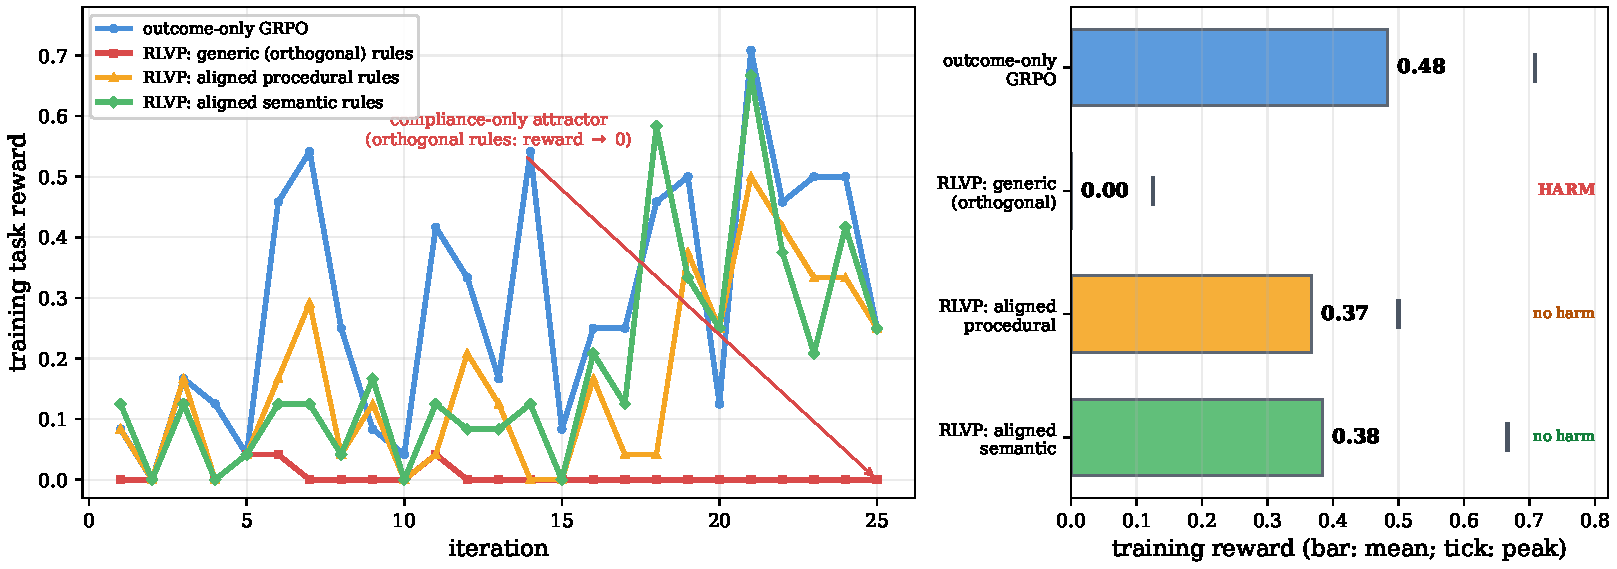
\includegraphics[width=\textwidth]{figures/fig_tau2_collapse.pdf}
\caption{\textbf{The coverage gradient on $\tau$-bench airline.} \emph{Left:} training reward for four signals. Outcome-only learns the benchmark; generic rules orthogonal to the reward collapse into the inaction trap; policy-derived procedural and verifiable-semantic rules (with early annealing) do not. \emph{Right:} mean reward per tier (bars) with peak (ticks). Misaligned rules harm; aligned rules remove the harm and nearly reach outcome-only's peak, but neither beats it. The residual gap is intent.}
\label{fig:tau2}
\end{figure}

\begin{figure}[tbp]
\centering
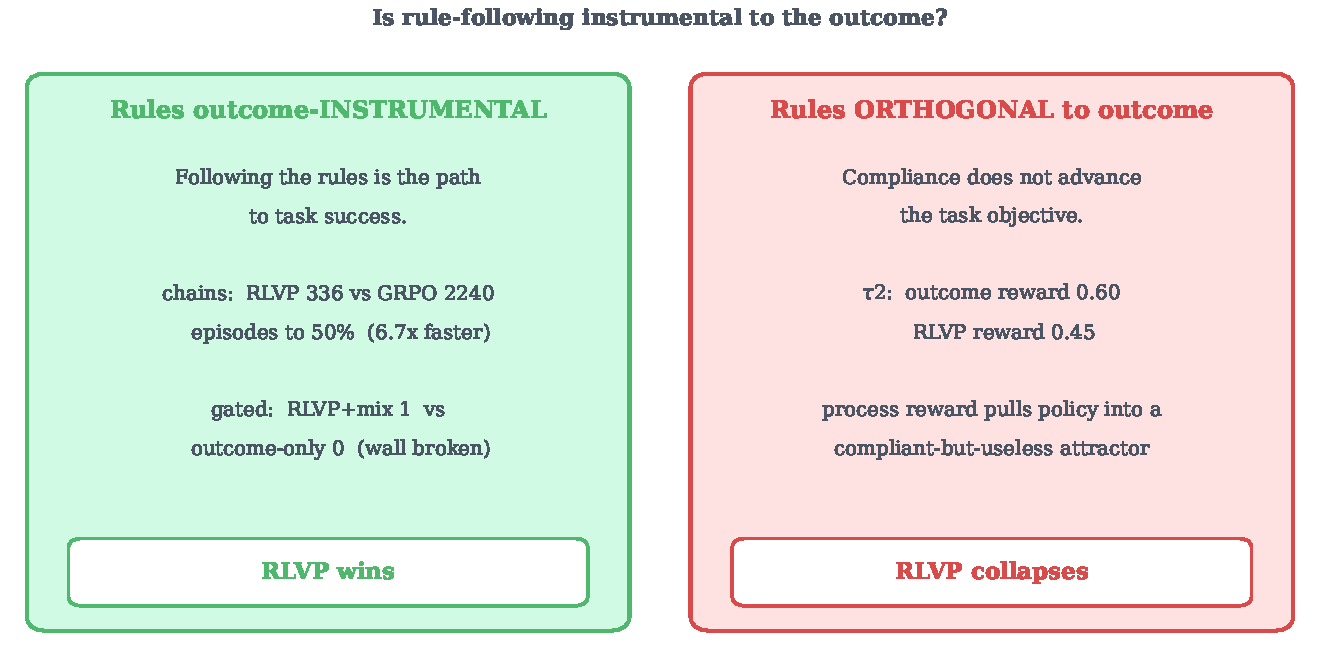
\includegraphics[width=0.96\textwidth]{figures/fig_boundary.pdf}
\caption{\textbf{The boundary on one axis: are the rules outcome-instrumental?} When the verifiable rules are aligned with what success requires (chained and gated tasks: the workflow \emph{is} the task), the process channel converts compliance into large outcome gains. When orthogonal to the reward ($\tau$-bench, generic rules), the same machinery optimizes compliance into a degenerate policy.}
\label{fig:boundary}
\end{figure}

\subsection{A learned critic relocates the hack}
\label{app:critic}

If verifiable rules cannot reach intent, why not let the policy judge itself, in the lineage of self-rewarding LMs and RLAIF~\citep{selfreward,rlaif,constitutional,llmjudge}? We use the critic as the \emph{same model} as the policy (no larger judge), so any signal is genuine on-policy self-reflection. Across two axes---whether a verifiable rule is cheaply specifiable, and whether the on-policy critic can detect the violation (Figure~\ref{fig:selfcritique})---the learned critic is a poor training reward in every quadrant. As a detector, blind self-critique flags surface-evident violations but is essentially blind to stateful-bookkeeping norms (did it read \emph{this} file before overwriting it) even when handed the rules, and the blind spot is structural (per-rule recall stays near zero as the critic scales). As a reward in the all-fail regime (Table~\ref{tab:sc-train}), a deterministic rule with identical credit structure is decisive on every seed while the self-critic---\emph{with perfect recall} against the rule oracle---is inert; a \emph{frozen} critic fails identically, isolating the cause as the critic's $\sim$6\% false-positive rate, not its non-stationarity. At the intent frontier (Table~\ref{tab:sc-tau2}) the self-critic is a useful \emph{offline} detector yet collapses as a training reward. Defining the penalized target by a learned proxy relocates the credit-assignment problem into the proxy, which the policy then games---the mechanism behind design rule~4. Verifiability is what makes the dense channel safe to optimize.

\begin{figure}[tbp]
\centering
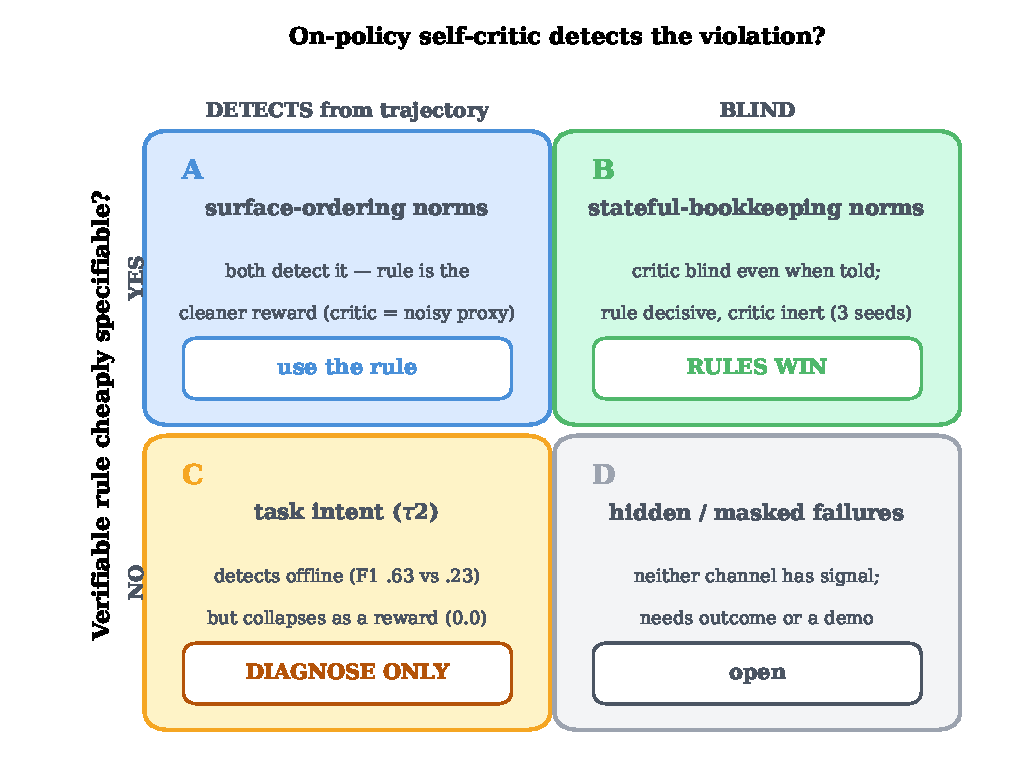
\includegraphics[width=0.72\textwidth]{figures/fig_selfcritique_2x2.pdf}
\caption{\textbf{When a verifiable rule beats a same-model self-critic, and when neither trains.} Axes: whether a verifiable rule is cheaply specifiable, and whether the on-policy critic can detect the violation. The learned critic is a poor training reward in every quadrant; its only robust use is offline diagnosis at the intent frontier.}
\label{fig:selfcritique}
\end{figure}

\begin{table}[tbp]
\centering
\caption{\textbf{A deterministic rule beats a same-model self-critic as a dense reward}, in the all-fail regime (consumer-service domain, 1.7B, three seeds; late-training mean $\pm$ std). Rule and critics share the identical penalty-only credit structure; the critic additionally has \emph{perfect recall} against the rule oracle. The rule is decisive every seed; the critics are inert. The \emph{frozen} (stationary) critic fails like the live one, isolating the cause as the critic's $\sim$6\% false-positive imprecision rather than non-stationarity.}
\label{tab:sc-train}
\small
\begin{tabular}{lccc}
\toprule
process reward & detection (P/R) & violations/episode & task success \\
\midrule
rule penalty (deterministic) & $1.00/1.00$ & $\mathbf{0.38 \pm 0.44}$ & $\mathbf{0.33 \pm 0.47}$ \\
self-critic, live (co-evolving) & $0.94/1.00$ & $0.94 \pm 0.05$ & $0.00$ \\
self-critic, frozen (stationary) & $0.94/1.00$ & $0.93 \pm 0.02$ & $0.00$ \\
\bottomrule
\end{tabular}

\vspace{0.8em}

\caption{\textbf{Self-critique is a usable intent \emph{detector} but a failed intent \emph{reward}} ($\tau$-bench airline, Qwen3-4B). \emph{Left:} as a failure predictor on rule-clean (intent) failures the self-critic far exceeds the verifiable semantic rules (3 rollout seeds). \emph{Right:} as the dense training reward the same self-critique collapses, while outcome-only and the rules both learn (training reward, early$\to$late; 20 iterations).}
\label{tab:sc-tau2}
\small
\begin{tabular}{lc@{\hskip 2.5em}lc}
\toprule
\multicolumn{2}{c}{\emph{offline: failure prediction}} & \multicolumn{2}{c}{\emph{trained as reward}} \\
channel & F1 & channel & reward (early$\to$late) \\
\midrule
semantic rules & $0.23 \pm 0.06$ & outcome-only & $0.09 \to \mathbf{0.50}$ \\
blind self-critique & $\mathbf{0.63 \pm 0.02}$ & semantic rules & $0.10 \to 0.35$ \\
 & & blind self-critique & $0.01 \to \mathbf{0.00}$ \\
\bottomrule
\end{tabular}
\end{table}



\section{Setting-by-Setting Summary}
\label{app:settings}

Table~\ref{tab:settings} collects the five settings studied across the paper against the three properties the variance account cares about---does a verifiable signal finer than the outcome exist, is it un-gameable, and are its intermediate values reachable---together with the observed outcome. Help appears only when a reachable, un-gameable signal is available; a penalty on always-sampled bad actions satisfies this on every row where it applies, while a progress potential does so only where partial progress is reachable.

\begin{table}[tbp]
\centering
\caption{\textbf{The five settings studied, summarized against the variance account.} Each row is a domain. The three middle columns are the conditions the account cares about: does a verifiable signal finer than the outcome exist, is it un-gameable, and are its intermediate values reachable. ``\cmark/\xmark'' marks the condition that decides the row. A dense signal helps only when all three hold; this table organizes the settings rather than predicting them.}
\label{tab:settings}
\small
\renewcommand{\arraystretch}{1.25}
\begin{tabular}{@{}p{2.9cm}p{2.0cm}cccp{1.6cm}p{2.7cm}@{}}
\toprule
\textbf{Setting} & \textbf{Domain / model} & \textbf{Finer $\Phi$?} & \textbf{Un-game?} & \textbf{Reach?} & \textbf{Verdict} & \textbf{Observed} \\
\midrule
Theorem proving (progress) & Lean miniF2F 30B, synth.\ 4B & \cmark & \cmark & \cmark & \textbf{help} & dead updates $\to 0$, dense gradient \\
System admin (harm) & TerminalBench 4B & \cmark & \cmark & \cmark & \textbf{help} (harm axis) & $\sim$6$\times$ fewer violations, equal success \\
Lean signal sweep (controlled) & miniF2F 30B & varies & \textbf{varies} & \cmark & per configuration & pure penalty dies, penalty-free survive \\
Customer service (intent) & $\tau$-bench airline 4B & \xmark & --- & --- & \textbf{no help} & rules match, never beat outcome \\
Software repair & SWE-bench 30B & 1/3 only & --- & \xmark & \textbf{no help} & $0\%$ solve, all rollouts $\Phi{=}0$ \\
\bottomrule
\end{tabular}
\end{table}

